\section{The SMEFT description of \texorpdfstring{\ggHH}{ggHH} production}
\label{sec:framework}

In the SMEFT the Higgs boson is part of an $SU(2)$ doublet with the same quantum numbers as in the SM, with the electroweak symmetry breaking being linearly realized, and the effects of new physics organized as a power series in $1/\Lambda$ according to canonical dimensions~\cite{Buchalla:2018yce, Heinrich:2022huh}. This work uses the available \texttt{ggHH\_SMEFT} implementation of \texttt{Powheg-Box-V2}~\cite{powheg1,powheg2,powheg3,Heinrich:2023rsd}, where the relevant terms for \ggHH production is given by the commonly used Warsaw basis:
\begin{equation}\label{eq:smeftL}
\begin{split}
    \mathcal{L}_\text{SMEFT}^\HH=& \frac{c_{\PH\Box}}{\Lambda^2}(\phi^\dagger\phi)\Box(\phi^\dagger\phi) + \frac{c_{\PH D}}{\Lambda^2}(\phi^\dagger D_\mu\phi)^*(\phi^\dagger D^\mu \phi) + \frac{c_\PH}{\Lambda^2}(\phi^\dagger\phi)^3 \\
     +&  \frac{c_{u\PH}}{\Lambda^2}(\phi^\dagger\phi\bar{Q}_L\tilde{\phi}\PQt_R + h.c.) +\frac{c_{\PH G}}{\Lambda^2}\phi^\dagger\phi G_{\mu\nu}^a G^{\mu\nu,a} \\
      +& \frac{c_{\PQt G}}{\Lambda^2}(\bar{Q}_L\sigma^{\mu\nu}T^a G^a_{\mu\nu}\tilde{\phi}\PQt_R + h.c.)\\
      +& \frac{c_{Q\PQt}^{(1)}}{\Lambda^2}\bar{Q}_L\gamma^\mu Q_L \bar{\PQt}_R\gamma_\mu \PQt_R + \frac{c_{Q\PQt}^{(8)}}{\Lambda^2}\bar{Q}_L\gamma^\mu T^a Q_L \bar{\PQt}_R \gamma_\mu T^a \PQt_R \\
      +& \frac{c_{QQ}^{(1)}}{\Lambda^2}\bar{Q}_L\gamma^\mu Q_L \bar{Q}_L\gamma_\mu Q_L + \frac{c_{QQ}^{(8)}}{\Lambda^2}\bar{Q}_L\gamma^\mu T^a Q_L \bar{Q}_L\gamma_\mu T^a Q_L\\
      +& \frac{c_{\PQt\PQt}}{\Lambda^2}\bar{\PQt}_R\gamma^\mu \PQt_R \bar{\PQt}_R\gamma_\mu \PQt_R.
\end{split}
\end{equation}
The set of dimension-6 operators described in this Lagrangian separates into two classes: \emph{leading} operators, with Wilson coefficients $\{c_{\PH\Box},\,c_{\PH D},\,c_\PH,\,c_{u\PH},\,c_{\PH G}\}$, and \emph{subleading} ones, with $\{c_{\PQt G},\,c_{Q\PQt}^{(1)},\,c_{Q\PQt}^{(8)},\,c_{QQ}^{(1)},\,c_{QQ}^{(8)},\,c_{\PQt\PQt}\}$. By "subleading" we mean operators that induce additional loops to the diagrams, hence carrying an implicit extra loop factor $L=(16\pi^2)^{-1}$~\cite{Heinrich:2023rsd}. The coefficients $c_{QQ}^{(1)}$ and $c_{\PQt\PQt}$ are combined into a single parameter $c_{QQ\PQt\PQt}=c_{QQ}^{(1)}+c_{\PQt\PQt}$, as their contributions to the amplitude factorize, and the kinetic coefficients are combined in the usual way as $c_{\PH\mathrm{kin}}=c_{\PH\Box}-\frac{1}{4}c_{\PH D}$. A point in the parameter space is therefore fixed by
\begin{equation}
\mathbf{c}^{\text{SMEFT}}=\{c_\PH,\,c_{\PH \mathrm{kin}},\,c_{u\PH},\,c_{\PH G},\,c_{\PQt G},\,c_{Q\PQt}^{(1)},\,c_{Q\PQt}^{(8)},\,c_{QQ\PQt\PQt},\,c_{QQ}^{(8)}\}\;,
\label{eq:smeftpoint}
\end{equation}
with the SM recovered when all Wilson coefficients vanish.



%At LO \ggHH proceeds through the box and triangle topologies, to which  correspond to the anomalous couplings of the Higgs EFT (HEFT), the non-linear framework in which the same process is modeled in Refs.~\cite{HEFT1,HHMatrix_R5, ELR_R5}.

The diagrams generated with the leading operators produce the usual SMEFT-HEFT naive translation as pointed in Ref.~\cite{Alasfar:2023xpc}, which allows us to connect, to some extent, the SMEFT modeling in this note with that presented in Refs.~\cite{HEFT1,HHMatrix_R5,ELR_R5}. On the other hand, the insertion of chromomagnetic and four-fermion operators lead to the inclusion of several additional graphs, as described in Ref.\cite{Heinrich:2023rsd}. Fig.~\ref{fig:feymnhh_subleading} exhibits two diagrams included with the addition of such operators, where no correspondence can be traced with the current HEFT implementations, since this would require the inclusion of higher-order operators in the chiral expansion used in such description. 

\begin{figure}[t]
    \centering
    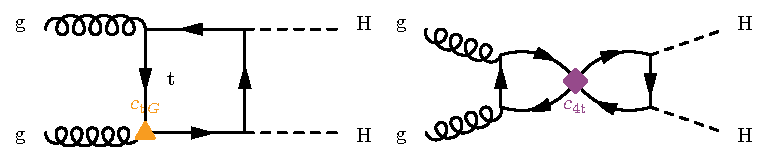
\includegraphics[width=\textwidth]{Diagrams/pdf/subleading}
    \caption{Representative Feynman diagrams induced by the subleading dimension-6 operators of Eq.~\eqref{eq:smeftL}~\cite{DiNoi:2024fdz}. Left: the chromomagnetic operator $c_{\PQt G}$ modifies the top--gluon vertex, marked by the triangle. Right: the four-fermion operators, collectively denoted $c_{4\PQt}$ and comprising $c_{Q\PQt}^{(1)}$, $c_{Q\PQt}^{(8)}$, $c_{QQ\PQt\PQt}$ and $c_{QQ}^{(8)}$, enter through the contact interaction between two top-quark loops, marked by the diamond.}
    \label{fig:feymnhh_subleading}
\end{figure}
